% Default to the notebook output style
% Inherit from the specified cell style.
\documentclass[11pt]{article}
  \usepackage[T1]{fontenc}
  % Nicer default font (+ math font) than Computer Modern for most use cases
  \usepackage{mathpazo}
  % Basic figure setup, for now with no caption control since it's done
  % automatically by Pandoc (which extracts ![](path) syntax from Markdown).
  \usepackage{graphicx}
  % We will generate all images so they have a width \maxwidth. This means
  % that they will get their normal width if they fit onto the page, but
  % are scaled down if they would overflow the margins.
  \makeatletter
  \def\maxwidth{\ifdim\Gin@nat@width>\linewidth\linewidth
  \else\Gin@nat@width\fi}
  \makeatother
  \let\Oldincludegraphics\includegraphics
  % Set max figure width to be 80% of text width, for now hardcoded.
  \renewcommand{\includegraphics}[1]{\Oldincludegraphics[width=.8\maxwidth]{#1}}
  % Ensure that by default, figures have no caption (until we provide a
  % proper Figure object with a Caption API and a way to capture that
  % in the conversion process - todo).
  \usepackage{caption}
  \DeclareCaptionLabelFormat{nolabel}{}
  \captionsetup{labelformat=nolabel}
  \usepackage{adjustbox} % Used to constrain images to a maximum size
  \usepackage{xcolor} % Allow colors to be defined
  \usepackage{enumerate} % Needed for markdown enumerations to work
  \usepackage{geometry} % Used to adjust the document margins
  \usepackage{amsmath} % Equations
  \usepackage{amssymb} % Equations
  \usepackage{textcomp} % defines textquotesingle
  % Hack from http://tex.stackexchange.com/a/47451/13684:
  \AtBeginDocument{%
      \def\PYZsq{\textquotesingle}% Upright quotes in Pygmentized code
  }
  \usepackage{upquote} % Upright quotes for verbatim code
  \usepackage{eurosym} % defines \euro
  \usepackage[mathletters]{ucs} % Extended unicode (utf-8) support
  \usepackage[utf8x]{inputenc} % Allow utf-8 characters in the tex document
  \usepackage{fancyvrb} % verbatim replacement that allows latex
  \usepackage{grffile} % extends the file name processing of package graphics
                       % to support a larger range
  % The hyperref package gives us a pdf with properly built
  % internal navigation ('pdf bookmarks' for the table of contents,
  % internal cross-reference links, web links for URLs, etc.)
  \usepackage{hyperref}
  \usepackage{longtable} % longtable support required by pandoc >1.10
  \usepackage{booktabs}  % table support for pandoc > 1.12.2
  \usepackage[inline]{enumitem} % IRkernel/repr support (it uses the enumerate* environment)
  \usepackage[normalem]{ulem} % ulem is needed to support strikethroughs (\sout)
                              % normalem makes italics be italics, not underlines
  \usepackage{mathrsfs}
  \usepackage{titling}
  \usepackage{fancyvrb}
  \usepackage{fvextra}
    % Colors for the hyperref package
    \definecolor{urlcolor}{rgb}{0,.145,.698}
    \definecolor{linkcolor}{rgb}{.71,0.21,0.01}
    \definecolor{citecolor}{rgb}{.12,.54,.11}

    % ANSI colors
    \definecolor{ansi-black}{HTML}{3E424D}
    \definecolor{ansi-black-intense}{HTML}{282C36}
    \definecolor{ansi-red}{HTML}{E75C58}
    \definecolor{ansi-red-intense}{HTML}{B22B31}
    \definecolor{ansi-green}{HTML}{00A250}
    \definecolor{ansi-green-intense}{HTML}{007427}
    \definecolor{ansi-yellow}{HTML}{DDB62B}
    \definecolor{ansi-yellow-intense}{HTML}{B27D12}
    \definecolor{ansi-blue}{HTML}{208FFB}
    \definecolor{ansi-blue-intense}{HTML}{0065CA}
    \definecolor{ansi-magenta}{HTML}{D160C4}
    \definecolor{ansi-magenta-intense}{HTML}{A03196}
    \definecolor{ansi-cyan}{HTML}{60C6C8}
    \definecolor{ansi-cyan-intense}{HTML}{258F8F}
    \definecolor{ansi-white}{HTML}{C5C1B4}
    \definecolor{ansi-white-intense}{HTML}{A1A6B2}
    \definecolor{ansi-default-inverse-fg}{HTML}{FFFFFF}
    \definecolor{ansi-default-inverse-bg}{HTML}{000000}

    % commands and environments needed by pandoc snippets
    % extracted from the output of `pandoc -s`
    \providecommand{\tightlist}{%
      \setlength{\itemsep}{0pt}\setlength{\parskip}{0pt}}
    \DefineVerbatimEnvironment{Highlighting}{Verbatim}{commandchars=\\\{\}}
    % Add ',fontsize=\small' for more characters per line
    \newenvironment{Shaded}{}{}
    \newcommand{\KeywordTok}[1]{\textcolor[rgb]{0.00,0.44,0.13}{\textbf{{#1}}}}
    \newcommand{\DataTypeTok}[1]{\textcolor[rgb]{0.56,0.13,0.00}{{#1}}}
    \newcommand{\DecValTok}[1]{\textcolor[rgb]{0.25,0.63,0.44}{{#1}}}
    \newcommand{\BaseNTok}[1]{\textcolor[rgb]{0.25,0.63,0.44}{{#1}}}
    \newcommand{\FloatTok}[1]{\textcolor[rgb]{0.25,0.63,0.44}{{#1}}}
    \newcommand{\CharTok}[1]{\textcolor[rgb]{0.25,0.44,0.63}{{#1}}}
    \newcommand{\StringTok}[1]{\textcolor[rgb]{0.25,0.44,0.63}{{#1}}}
    \newcommand{\CommentTok}[1]{\textcolor[rgb]{0.38,0.63,0.69}{\textit{{#1}}}}
    \newcommand{\OtherTok}[1]{\textcolor[rgb]{0.00,0.44,0.13}{{#1}}}
    \newcommand{\AlertTok}[1]{\textcolor[rgb]{1.00,0.00,0.00}{\textbf{{#1}}}}
    \newcommand{\FunctionTok}[1]{\textcolor[rgb]{0.02,0.16,0.49}{{#1}}}
    \newcommand{\RegionMarkerTok}[1]{{#1}}
    \newcommand{\ErrorTok}[1]{\textcolor[rgb]{1.00,0.00,0.00}{\textbf{{#1}}}}
    \newcommand{\NormalTok}[1]{{#1}}

    % Additional commands for more recent versions of Pandoc
    \newcommand{\ConstantTok}[1]{\textcolor[rgb]{0.53,0.00,0.00}{{#1}}}
    \newcommand{\SpecialCharTok}[1]{\textcolor[rgb]{0.25,0.44,0.63}{{#1}}}
    \newcommand{\VerbatimStringTok}[1]{\textcolor[rgb]{0.25,0.44,0.63}{{#1}}}
    \newcommand{\SpecialStringTok}[1]{\textcolor[rgb]{0.73,0.40,0.53}{{#1}}}
    \newcommand{\ImportTok}[1]{{#1}}
    \newcommand{\DocumentationTok}[1]{\textcolor[rgb]{0.73,0.13,0.13}{\textit{{#1}}}}
    \newcommand{\AnnotationTok}[1]{\textcolor[rgb]{0.38,0.63,0.69}{\textbf{\textit{{#1}}}}}
    \newcommand{\CommentVarTok}[1]{\textcolor[rgb]{0.38,0.63,0.69}{\textbf{\textit{{#1}}}}}
    \newcommand{\VariableTok}[1]{\textcolor[rgb]{0.10,0.09,0.49}{{#1}}}
    \newcommand{\ControlFlowTok}[1]{\textcolor[rgb]{0.00,0.44,0.13}{\textbf{{#1}}}}
    \newcommand{\OperatorTok}[1]{\textcolor[rgb]{0.40,0.40,0.40}{{#1}}}
    \newcommand{\BuiltInTok}[1]{{#1}}
    \newcommand{\ExtensionTok}[1]{{#1}}
    \newcommand{\PreprocessorTok}[1]{\textcolor[rgb]{0.74,0.48,0.00}{{#1}}}
    \newcommand{\AttributeTok}[1]{\textcolor[rgb]{0.49,0.56,0.16}{{#1}}}
    \newcommand{\InformationTok}[1]{\textcolor[rgb]{0.38,0.63,0.69}{\textbf{\textit{{#1}}}}}
    \newcommand{\WarningTok}[1]{\textcolor[rgb]{0.38,0.63,0.69}{\textbf{\textit{{#1}}}}}


    % Define a nice break command that doesn't care if a line doesn't already
    % exist.
    \def\br{\hspace*{\fill} \\* }
    % Math Jax compatibility definitions
    \def\gt{>}
    \def\lt{<}
    \let\Oldtex\TeX
    \let\Oldlatex\LaTeX
    \renewcommand{\TeX}{\textrm{\Oldtex}}
    \renewcommand{\LaTeX}{\textrm{\Oldlatex}}
    % Document parameters
    % Document title
    \title{%
    Artificial Intelligence and Machine Learning\newline
    \large \newline Homework 3: Deep Learning
    }
    \author{Jeanpierre Francois S243920}
    % Pygments definitions

\makeatletter
\def\PY@reset{\let\PY@it=\relax \let\PY@bf=\relax%
    \let\PY@ul=\relax \let\PY@tc=\relax%
    \let\PY@bc=\relax \let\PY@ff=\relax}
\def\PY@tok#1{\csname PY@tok@#1\endcsname}
\def\PY@toks#1+{\ifx\relax#1\empty\else%
    \PY@tok{#1}\expandafter\PY@toks\fi}
\def\PY@do#1{\PY@bc{\PY@tc{\PY@ul{%
    \PY@it{\PY@bf{\PY@ff{#1}}}}}}}
\def\PY#1#2{\PY@reset\PY@toks#1+\relax+\PY@do{#2}}

\expandafter\def\csname PY@tok@w\endcsname{\def\PY@tc##1{\textcolor[rgb]{0.73,0.73,0.73}{##1}}}
\expandafter\def\csname PY@tok@c\endcsname{\let\PY@it=\textit\def\PY@tc##1{\textcolor[rgb]{0.25,0.50,0.50}{##1}}}
\expandafter\def\csname PY@tok@cp\endcsname{\def\PY@tc##1{\textcolor[rgb]{0.74,0.48,0.00}{##1}}}
\expandafter\def\csname PY@tok@k\endcsname{\let\PY@bf=\textbf\def\PY@tc##1{\textcolor[rgb]{0.00,0.50,0.00}{##1}}}
\expandafter\def\csname PY@tok@kp\endcsname{\def\PY@tc##1{\textcolor[rgb]{0.00,0.50,0.00}{##1}}}
\expandafter\def\csname PY@tok@kt\endcsname{\def\PY@tc##1{\textcolor[rgb]{0.69,0.00,0.25}{##1}}}
\expandafter\def\csname PY@tok@o\endcsname{\def\PY@tc##1{\textcolor[rgb]{0.40,0.40,0.40}{##1}}}
\expandafter\def\csname PY@tok@ow\endcsname{\let\PY@bf=\textbf\def\PY@tc##1{\textcolor[rgb]{0.67,0.13,1.00}{##1}}}
\expandafter\def\csname PY@tok@nb\endcsname{\def\PY@tc##1{\textcolor[rgb]{0.00,0.50,0.00}{##1}}}
\expandafter\def\csname PY@tok@nf\endcsname{\def\PY@tc##1{\textcolor[rgb]{0.00,0.00,1.00}{##1}}}
\expandafter\def\csname PY@tok@nc\endcsname{\let\PY@bf=\textbf\def\PY@tc##1{\textcolor[rgb]{0.00,0.00,1.00}{##1}}}
\expandafter\def\csname PY@tok@nn\endcsname{\let\PY@bf=\textbf\def\PY@tc##1{\textcolor[rgb]{0.00,0.00,1.00}{##1}}}
\expandafter\def\csname PY@tok@ne\endcsname{\let\PY@bf=\textbf\def\PY@tc##1{\textcolor[rgb]{0.82,0.25,0.23}{##1}}}
\expandafter\def\csname PY@tok@nv\endcsname{\def\PY@tc##1{\textcolor[rgb]{0.10,0.09,0.49}{##1}}}
\expandafter\def\csname PY@tok@no\endcsname{\def\PY@tc##1{\textcolor[rgb]{0.53,0.00,0.00}{##1}}}
\expandafter\def\csname PY@tok@nl\endcsname{\def\PY@tc##1{\textcolor[rgb]{0.63,0.63,0.00}{##1}}}
\expandafter\def\csname PY@tok@ni\endcsname{\let\PY@bf=\textbf\def\PY@tc##1{\textcolor[rgb]{0.60,0.60,0.60}{##1}}}
\expandafter\def\csname PY@tok@na\endcsname{\def\PY@tc##1{\textcolor[rgb]{0.49,0.56,0.16}{##1}}}
\expandafter\def\csname PY@tok@nt\endcsname{\let\PY@bf=\textbf\def\PY@tc##1{\textcolor[rgb]{0.00,0.50,0.00}{##1}}}
\expandafter\def\csname PY@tok@nd\endcsname{\def\PY@tc##1{\textcolor[rgb]{0.67,0.13,1.00}{##1}}}
\expandafter\def\csname PY@tok@s\endcsname{\def\PY@tc##1{\textcolor[rgb]{0.73,0.13,0.13}{##1}}}
\expandafter\def\csname PY@tok@sd\endcsname{\let\PY@it=\textit\def\PY@tc##1{\textcolor[rgb]{0.73,0.13,0.13}{##1}}}
\expandafter\def\csname PY@tok@si\endcsname{\let\PY@bf=\textbf\def\PY@tc##1{\textcolor[rgb]{0.73,0.40,0.53}{##1}}}
\expandafter\def\csname PY@tok@se\endcsname{\let\PY@bf=\textbf\def\PY@tc##1{\textcolor[rgb]{0.73,0.40,0.13}{##1}}}
\expandafter\def\csname PY@tok@sr\endcsname{\def\PY@tc##1{\textcolor[rgb]{0.73,0.40,0.53}{##1}}}
\expandafter\def\csname PY@tok@ss\endcsname{\def\PY@tc##1{\textcolor[rgb]{0.10,0.09,0.49}{##1}}}
\expandafter\def\csname PY@tok@sx\endcsname{\def\PY@tc##1{\textcolor[rgb]{0.00,0.50,0.00}{##1}}}
\expandafter\def\csname PY@tok@m\endcsname{\def\PY@tc##1{\textcolor[rgb]{0.40,0.40,0.40}{##1}}}
\expandafter\def\csname PY@tok@gh\endcsname{\let\PY@bf=\textbf\def\PY@tc##1{\textcolor[rgb]{0.00,0.00,0.50}{##1}}}
\expandafter\def\csname PY@tok@gu\endcsname{\let\PY@bf=\textbf\def\PY@tc##1{\textcolor[rgb]{0.50,0.00,0.50}{##1}}}
\expandafter\def\csname PY@tok@gd\endcsname{\def\PY@tc##1{\textcolor[rgb]{0.63,0.00,0.00}{##1}}}
\expandafter\def\csname PY@tok@gi\endcsname{\def\PY@tc##1{\textcolor[rgb]{0.00,0.63,0.00}{##1}}}
\expandafter\def\csname PY@tok@gr\endcsname{\def\PY@tc##1{\textcolor[rgb]{1.00,0.00,0.00}{##1}}}
\expandafter\def\csname PY@tok@ge\endcsname{\let\PY@it=\textit}
\expandafter\def\csname PY@tok@gs\endcsname{\let\PY@bf=\textbf}
\expandafter\def\csname PY@tok@gp\endcsname{\let\PY@bf=\textbf\def\PY@tc##1{\textcolor[rgb]{0.00,0.00,0.50}{##1}}}
\expandafter\def\csname PY@tok@go\endcsname{\def\PY@tc##1{\textcolor[rgb]{0.53,0.53,0.53}{##1}}}
\expandafter\def\csname PY@tok@gt\endcsname{\def\PY@tc##1{\textcolor[rgb]{0.00,0.27,0.87}{##1}}}
\expandafter\def\csname PY@tok@err\endcsname{\def\PY@bc##1{\setlength{\fboxsep}{0pt}\fcolorbox[rgb]{1.00,0.00,0.00}{1,1,1}{\strut ##1}}}
\expandafter\def\csname PY@tok@kc\endcsname{\let\PY@bf=\textbf\def\PY@tc##1{\textcolor[rgb]{0.00,0.50,0.00}{##1}}}
\expandafter\def\csname PY@tok@kd\endcsname{\let\PY@bf=\textbf\def\PY@tc##1{\textcolor[rgb]{0.00,0.50,0.00}{##1}}}
\expandafter\def\csname PY@tok@kn\endcsname{\let\PY@bf=\textbf\def\PY@tc##1{\textcolor[rgb]{0.00,0.50,0.00}{##1}}}
\expandafter\def\csname PY@tok@kr\endcsname{\let\PY@bf=\textbf\def\PY@tc##1{\textcolor[rgb]{0.00,0.50,0.00}{##1}}}
\expandafter\def\csname PY@tok@bp\endcsname{\def\PY@tc##1{\textcolor[rgb]{0.00,0.50,0.00}{##1}}}
\expandafter\def\csname PY@tok@fm\endcsname{\def\PY@tc##1{\textcolor[rgb]{0.00,0.00,1.00}{##1}}}
\expandafter\def\csname PY@tok@vc\endcsname{\def\PY@tc##1{\textcolor[rgb]{0.10,0.09,0.49}{##1}}}
\expandafter\def\csname PY@tok@vg\endcsname{\def\PY@tc##1{\textcolor[rgb]{0.10,0.09,0.49}{##1}}}
\expandafter\def\csname PY@tok@vi\endcsname{\def\PY@tc##1{\textcolor[rgb]{0.10,0.09,0.49}{##1}}}
\expandafter\def\csname PY@tok@vm\endcsname{\def\PY@tc##1{\textcolor[rgb]{0.10,0.09,0.49}{##1}}}
\expandafter\def\csname PY@tok@sa\endcsname{\def\PY@tc##1{\textcolor[rgb]{0.73,0.13,0.13}{##1}}}
\expandafter\def\csname PY@tok@sb\endcsname{\def\PY@tc##1{\textcolor[rgb]{0.73,0.13,0.13}{##1}}}
\expandafter\def\csname PY@tok@sc\endcsname{\def\PY@tc##1{\textcolor[rgb]{0.73,0.13,0.13}{##1}}}
\expandafter\def\csname PY@tok@dl\endcsname{\def\PY@tc##1{\textcolor[rgb]{0.73,0.13,0.13}{##1}}}
\expandafter\def\csname PY@tok@s2\endcsname{\def\PY@tc##1{\textcolor[rgb]{0.73,0.13,0.13}{##1}}}
\expandafter\def\csname PY@tok@sh\endcsname{\def\PY@tc##1{\textcolor[rgb]{0.73,0.13,0.13}{##1}}}
\expandafter\def\csname PY@tok@s1\endcsname{\def\PY@tc##1{\textcolor[rgb]{0.73,0.13,0.13}{##1}}}
\expandafter\def\csname PY@tok@mb\endcsname{\def\PY@tc##1{\textcolor[rgb]{0.40,0.40,0.40}{##1}}}
\expandafter\def\csname PY@tok@mf\endcsname{\def\PY@tc##1{\textcolor[rgb]{0.40,0.40,0.40}{##1}}}
\expandafter\def\csname PY@tok@mh\endcsname{\def\PY@tc##1{\textcolor[rgb]{0.40,0.40,0.40}{##1}}}
\expandafter\def\csname PY@tok@mi\endcsname{\def\PY@tc##1{\textcolor[rgb]{0.40,0.40,0.40}{##1}}}
\expandafter\def\csname PY@tok@il\endcsname{\def\PY@tc##1{\textcolor[rgb]{0.40,0.40,0.40}{##1}}}
\expandafter\def\csname PY@tok@mo\endcsname{\def\PY@tc##1{\textcolor[rgb]{0.40,0.40,0.40}{##1}}}
\expandafter\def\csname PY@tok@ch\endcsname{\let\PY@it=\textit\def\PY@tc##1{\textcolor[rgb]{0.25,0.50,0.50}{##1}}}
\expandafter\def\csname PY@tok@cm\endcsname{\let\PY@it=\textit\def\PY@tc##1{\textcolor[rgb]{0.25,0.50,0.50}{##1}}}
\expandafter\def\csname PY@tok@cpf\endcsname{\let\PY@it=\textit\def\PY@tc##1{\textcolor[rgb]{0.25,0.50,0.50}{##1}}}
\expandafter\def\csname PY@tok@c1\endcsname{\let\PY@it=\textit\def\PY@tc##1{\textcolor[rgb]{0.25,0.50,0.50}{##1}}}
\expandafter\def\csname PY@tok@cs\endcsname{\let\PY@it=\textit\def\PY@tc##1{\textcolor[rgb]{0.25,0.50,0.50}{##1}}}

\def\PYZbs{\char`\\}
\def\PYZus{\char`\_}
\def\PYZob{\char`\{}
\def\PYZcb{\char`\}}
\def\PYZca{\char`\^}
\def\PYZam{\char`\&}
\def\PYZlt{\char`\<}
\def\PYZgt{\char`\>}
\def\PYZsh{\char`\#}
\def\PYZpc{\char`\%}
\def\PYZdl{\char`\$}
\def\PYZhy{\char`\-}
\def\PYZsq{\char`\'}
\def\PYZdq{\char`\"}
\def\PYZti{\char`\~}
% for compatibility with earlier versions
\def\PYZat{@}
\def\PYZlb{[}
\def\PYZrb{]}
\makeatother
    % Exact colors from NB
    \definecolor{incolor}{rgb}{0.0, 0.0, 0.5}
    \definecolor{outcolor}{rgb}{0.545, 0.0, 0.0}
    % Prevent overflowing lines due to hard-to-break entities
    \sloppy
    % Setup hyperref package
    \hypersetup{
      breaklinks=true,  % so long urls are correctly broken across lines
      colorlinks=true,
      urlcolor=urlcolor,
      linkcolor=linkcolor,
      citecolor=citecolor,
      }
    % Slightly bigger margins than the latex defaults
    \geometry{verbose,tmargin=1in,bmargin=1in,lmargin=1in,rmargin=1in}
    \begin{document}
    \maketitle
    \begin{center}
      
\includegraphics{polito_logo.png}
    \end{center}
    \newpage

\section{Description}\label{description}
In this homework I explored the tip of the iceberg regarding deep learning and neural networks applications. \newline
The language used in this homework is python, the framework implemented is pytorch. \newline
The homework was written and run onto google's Colab platform. \newline
The images dataset used for training and testing the networks is the CIFAR100 imported from torchvision.\newline
Whithin the homework I worked with three different kinds of neural network:
\begin{enumerate}
  \item \hyperlink{oldnn}{Old neural network}
  \item \hyperlink{cnn}{Convolutional neural network}
  \item \hyperlink{resNet}{ResNet-18}
\end{enumerate}
\newpage

\section{Old Neural Networks}\label{oldnn}\hypertarget{oldnn}{}
The so called old neural network implemented is a simple traditional net, provided with forward and backward propagation, composed of three fully connected layers: two hidden and one for the classification.
The transformations comprohends a resize and a normalization of the input images with a batch size of 256.
The chosen solver is Adam with a learning rate of 0.0001. \newline
\begin{center}
  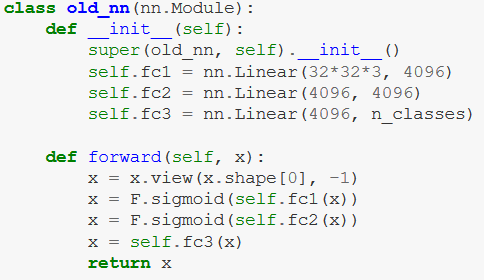
\includegraphics{1_class.png}
  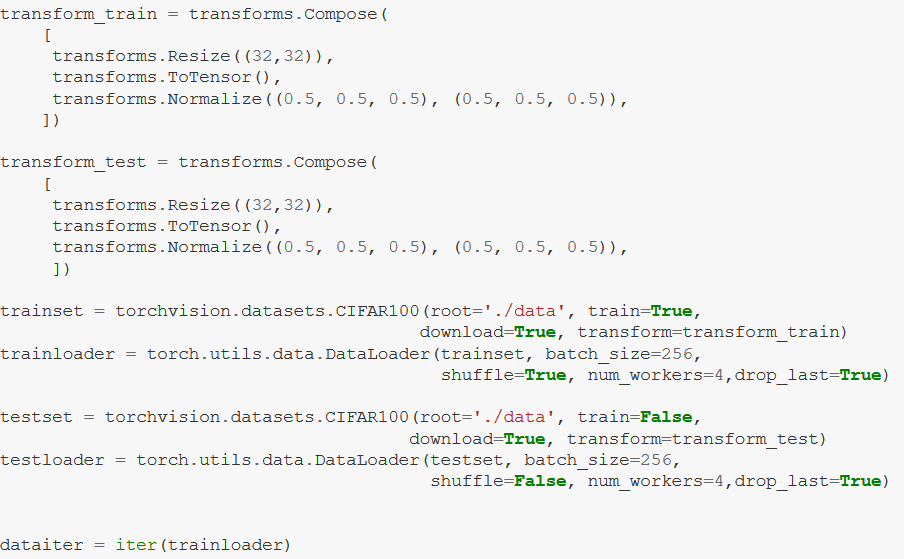
\includegraphics{1_tran.png} \newline
\end{center}
Storing at each epoch the accuracy and loss obtained, within 20 epochs I obtained a final score on the test set of 26\% with a loss of 2.680 in 4 minutes and 7 seconds as shown in the subsequent results.
\begin{center}
  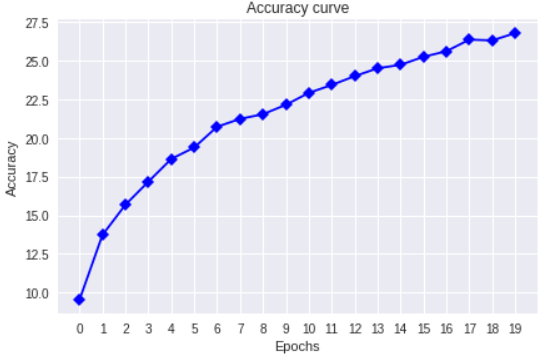
\includegraphics{1_acc.png}
  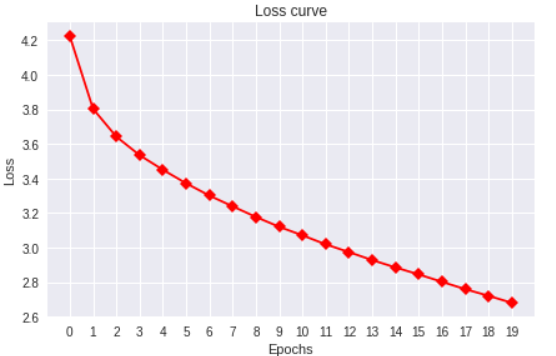
\includegraphics{1_loss.png}
\end{center}
Despite the simplicity of the deployed net I got an accuracy of 26\% that may seem low is still a pretty good result working with 100 classes, the starting chance was of 1\% and this neural network rose it up of 26 times, which is nice.
\newpage
\section{Convolutional Neural Networks}\label{cnn}\hypertarget{cnn}{}
Convolutional neural networks (cnn) are neural net applied to images where each hidden unit is connected to a small patch of the input and shares weights across space. This networks are capable of learning filters without prior knowledge. \newline
In this practice multiple different cnn have been tested.\newline
I trained the cnn from scratch using the various network configuration and data augmentation requested in the homework obtaining the following results. \newline
\begin{center}
    \begin{tabular}{ | l | l | l | l |}
    \hline
    Net configuration & Accuracy & Time & Loss \\ \hline
    2of6\_32/32/32/64 & 30\% & 00:04:30 & 2.116 \\ \hline
    3of6\_128/128/128/256 & 32\% & 00:06:17 & 0.149 \\ \hline
    3of6\_256/256/256/512 & 35\% & 00:14:12 & 0.076 \\ \hline
    3of6\_512/512/512/1024 & 36\% & 00:42:32 & 0.049 \\ \hline
    4of6\_a & 43\% & 00:06:31 & 0.122 \\ \hline
    4of6\_b & 44\% & 00:07:50 & 0.048 \\ \hline
    4of6\_c & 45\% & 00:06:30 & 0.641 \\ \hline
    5of6\_a & 35\% & 00:05:51 & 0.827 \\ \hline
    5of6\_b & 33\% & 00:06:20 & 2.101 \\ \hline
    Best cnn found & 58\% & 00:50:36 & 0.544 \\ \hline
    \end{tabular}
\end{center}
Every cnn deployed for the work share a similar base architecture: four convolutional layers, two fully connected with ReLu and max pooling strategies.
\subsection{2of6}
This is the first convolutional network deployed with a number of convolutional filters of 32/32/32/64. As we can see from the accuracy obtained it's way better in classifying CIFAR100's images than a simple neural network composed of fully connected layers as the one implemented in the previous \"old nn\".
\subsection{3of6}
The computational time grows as I increment the number of convolutional filters from 32/32/32/64 to 128/128/128/256, then again to 256/256/256/512 and finally to 512/512/512/1024. Incrementing the number of filters will result in a slow and slower learning. \newline
Regarding the accuracy scores on the test set I saw them grow less and less doubling the number of filters so I guess the accuracy improvement obtained by only adding filters is limited.
\subsection{4of6}
Applying batch normalization after each convolutional layer normalizes the flowing data in the whole network speeding up convergence. It results in an great increment in accuracy from the previous 32\% up to 43\%. \newline
Trying to use a wider fully connected layer (fc1 8096 neurons) brings a longer training time for a little improvement of around 1\% in accuracy but a strong decrease for the loss probably because it overfits onto training set. \newline
Dropout randomly sets neurons activations to zero during the training process to avoid overfitting and it increase slightly the accuracy but also the loss. \newline
4of6\_c was the best cnn configuration found among the proposed: \newline
\begin{center}
  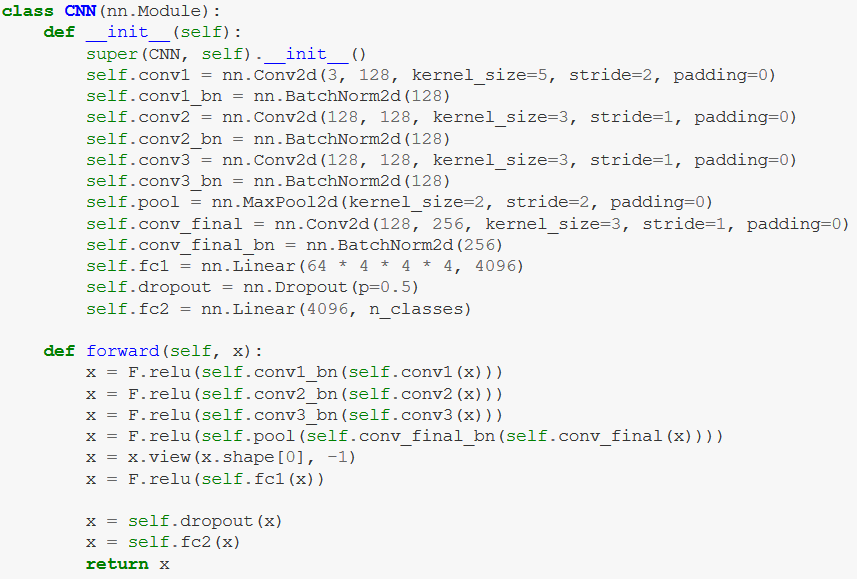
\includegraphics{2_class.png}\newline
  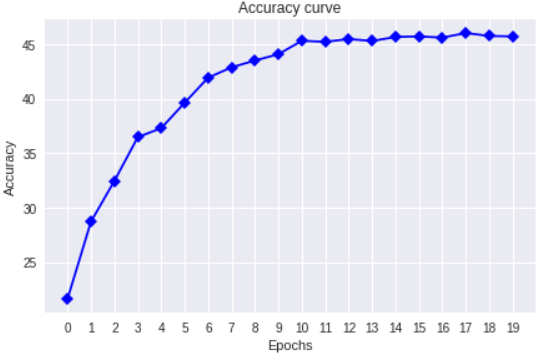
\includegraphics{2_acc.png}
  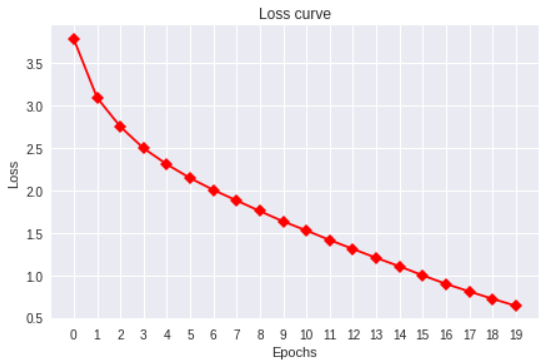
\includegraphics{2_loss.png}
\end{center}
\subsection{5of6}
Whith a limited dataset, data augmentation techniques comes in handy to limit overfitting on a small training set and, by changing input during training, let the network generalize better. \newline
In this case random horizontal flipping gave a better score and lower loss than random cropping probably because our dataset is composed of 32x32 rgb images and for the latter technique we have to first resize them to 40x40 and only then crop.
\subsection{Best cnn results}
By combying some of the techniques seen in the previous configurations while focusing on performance the best result I obtained, out of the ones tested, through applying batch normalization to every convolutional layer, dropout to limit overfitting, random horizontal flips as data augmentation, a number of filters of 512/512/512/1024 with a wider fully connected layer with 8096 neurons is 58\% of accuracy with a low loss as 0.544 with the following components: \newline
\begin{center}
  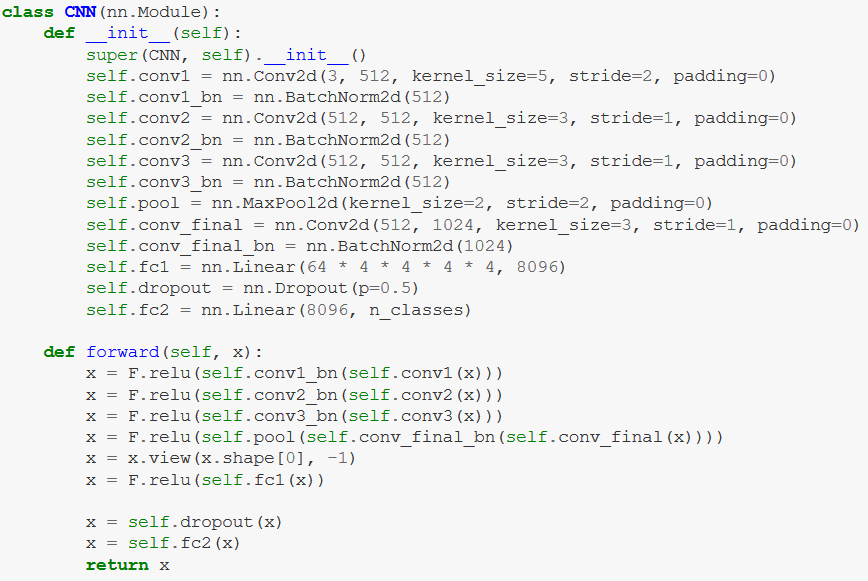
\includegraphics{best_cnn_class.png}
  %\includegraphics{best_cnn_tran.png}
  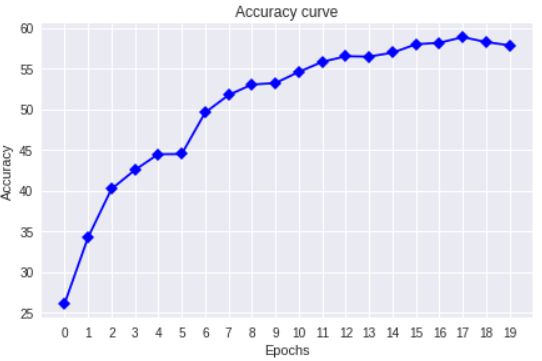
\includegraphics{best_cnn_acc.png}
  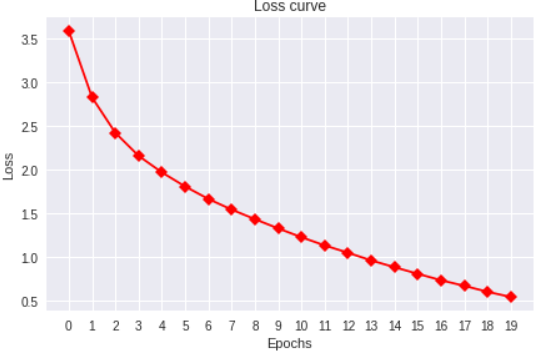
\includegraphics{best_cnn_loss.png}
\end{center}
\newpage
\section{ResNet-18}\label{resNet}\hypertarget{resNet}{}
ResNet architecture solves the problem of the vanishing gradient in ultra-deep networks, where accuracy gets saturated and then degrades rapidly, using residual functions. \newline
The one I used was ResNet-18-layer taken from pytorch framework, pretrained on imagenet, with horizontal random flip as data augmentation. \newline
\begin{center}
  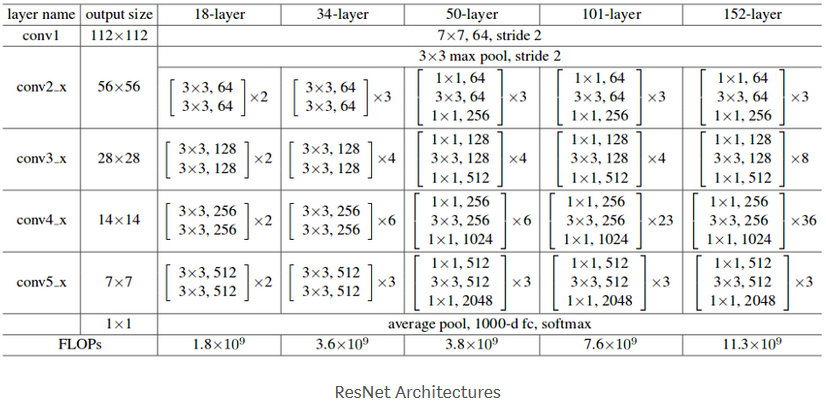
\includegraphics{3_class.png} \newline
  The ResNet-18 blocks are two layer deep \newline
  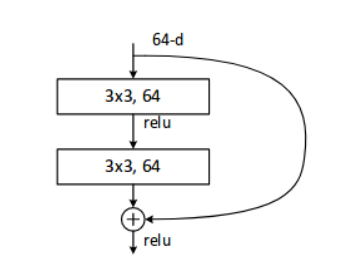
\includegraphics{3_class2.png} \newline
\end{center}
Even if its training is very slow, having it pretrained on the vast dataset of imagenet before finetunig it onto CIFAR100 for ten epochs resulted in really good scores. \newline
\begin{center}
    \begin{tabular}{ | l | l | l | l |}
    \hline
    Net configuration & Accuracy & Time & Loss \\ \hline
    6of6 & 79\% & 01:01:01 & 0.044 \\ \hline
  \end{tabular}
  \newline
  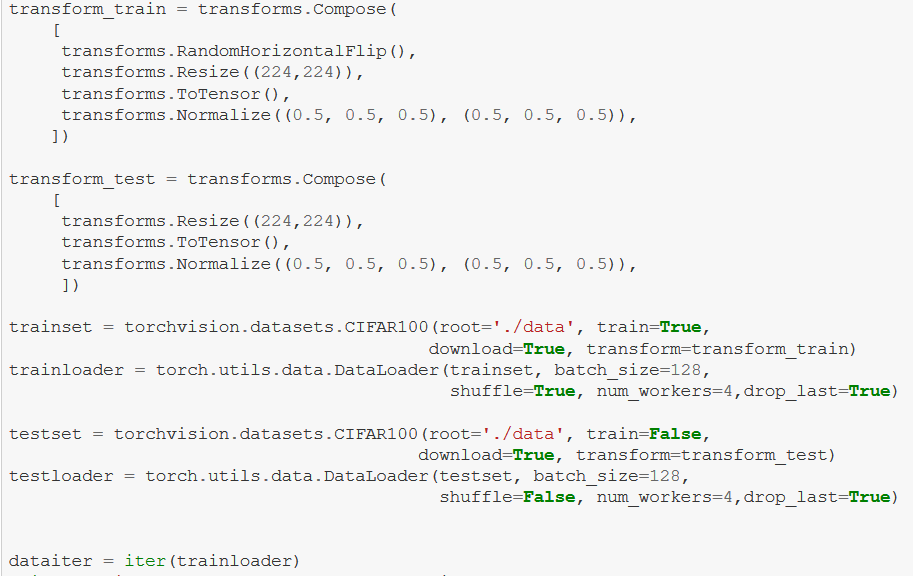
\includegraphics{3_tran.png}
  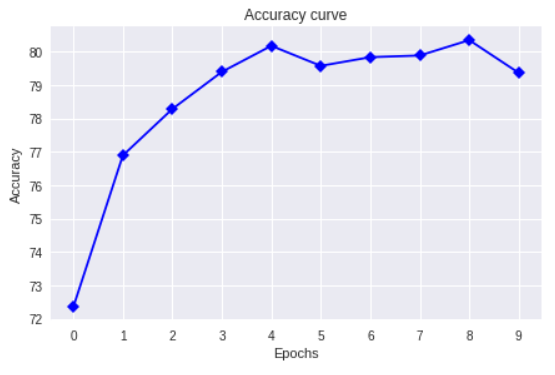
\includegraphics{3_acc.png}
  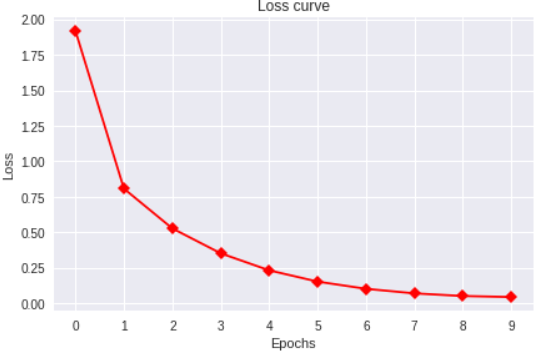
\includegraphics{3_loss.png}
\end{center}
ResNet gave the best results out of the tested networks not only because is a deeper cutting edge research network but also because it was pretrained on the vast imagenet database and only then finetuned on our CIFAR100.

%\section{Conclusions}\label{conclusions}\hypertarget{conclusions}{}
%Deep learning it's free real estate world for research at the moment where new discoveries are popping out day by day and a lot of publication are being made. \newline
%In the last fifteen years researchers came up with more and more effective ways to train deeper networks and the best approaches changes almost yearly. From using %sigmoid to ReLu, from wide fully connected only networks up to convolutional deep networks with residual functions. In this homework I had the opportunity to see with %my very eyes how big is the difference between old neural networks and cutting edge research one.

\end{document}
